\documentclass[10pt]{article}
\usepackage[margin=1in]{geometry}
\usepackage[T1]{fontenc}
\usepackage{lmodern,microtype}
\usepackage{amsmath,amssymb,amsthm,mathtools}
\usepackage{graphicx,booktabs,float}
\usepackage[hidelinks]{hyperref}
\usepackage{enumitem}
\usepackage{xcolor}
\usepackage[most]{tcolorbox}

\setlength{\parindent}{0pt}
\setlength{\parskip}{0.32em}
\setlength{\abovedisplayskip}{5pt plus 1pt minus 2pt}
\setlength{\belowdisplayskip}{5pt plus 1pt minus 2pt}
\setlength{\abovedisplayshortskip}{3pt plus 1pt}
\setlength{\belowdisplayshortskip}{3pt plus 1pt}
\setlist[itemize]{leftmargin=1.25em,itemsep=0.08em,topsep=0.18em}
\setlist[enumerate]{leftmargin=1.45em,itemsep=0.08em,topsep=0.18em}

\definecolor{questionink}{HTML}{24344D}
\definecolor{questionline}{HTML}{5479A8}
\definecolor{questionwash}{HTML}{F3F6FA}
\newtcolorbox{questionbox}{
  enhanced,
  colback=questionwash,
  colframe=questionline!42,
  boxrule=0.45pt,
  arc=2mm,
  left=3.2mm,
  right=3.2mm,
  top=2.5mm,
  bottom=2.3mm,
  borderline west={2.2pt}{0pt}{questionline},
  before skip=0.5em,
  after skip=0.55em
}

\newtheoremstyle{compact}
  {5pt}{5pt}{\itshape}{}{}{.}{0.45em}{}
\theoremstyle{compact}
\newtheorem{theorem}{Theorem}
\newtheorem{proposition}{Proposition}

\newcommand{\E}{\mathbb E}
\newcommand{\Var}{\operatorname{Var}}

\begin{document}

\begin{center}
{\LARGE\bfseries The Finite Response Structure of LLM Scaling Laws}\par
\vspace{0.18em}
{\large Apparent takeoff as a resolved, two-stage generalization process}\par
\vspace{0.52em}
{Jonathan R. Landers \qquad July 2026}
\end{center}
\vspace{0.1em}

\begin{abstract}
Scaling laws describe how far a learning system moves, but not how a new
regime arrives. We treat LLM takeoff as a finite response: the cumulative
arrival of improvement is a step response \(F_t\), and its finite difference
\(\kappa_t\) is a takeoff kernel. A delta kernel is instantaneous; a broad or
multilobed kernel carries temporal structure that a terminal exponent or
changepoint cannot retain. We test this distinction in a controlled
grokking-style Transformer trained on modular addition. Across six independent
seeds, the late rise from 50 to 90 percent held-out accuracy occupies
600--1,250 optimizer updates, or 12--25 resolved checkpoint intervals. More
strikingly, a two-response mixture predicts held-out checkpoints better than
either a step or one smooth response in every seed. Roughly 30 percent of the
fitted response arrives in an early component and 70 percent in a later,
sharper component. The apparent takeoff is therefore not the whole event; it
is the second lobe of a longer response. A separate modal test finds no need
for two exponential settling modes, so the evidence supports two transition
stages without yet identifying two physical mechanisms.
\end{abstract}

\section*{1. The part a scaling law leaves out}

A scaling law is deliberately forgetful. It compresses a family of models,
datasets, or training runs into an asymptotic relation, often with remarkable
predictive power \cite{kaplan2020,hoffmann2022}. But a terminal rate does not
say how that rate became visible. Two trajectories may share the same
eventual exponent while one turns on immediately, another gathers momentum
over thousands of updates, and a third arrives through several overlapping
stages.

This missing temporal information matters most when a curve is described as
\emph{takeoff}. A late transition can look sudden simply because its waiting
time is long compared with its final rise. That contrast is visually real,
but it does not make the rise instantaneous. Nor does the location of a
changepoint tell us whether earlier, smaller components were already delivering
part of the eventual gain.

The finite-response view separates three questions:
\begin{questionbox}
\begin{enumerate}[
  leftmargin=1.8em,
  label=\textcolor{questionline}{\bfseries\arabic*.},
  labelsep=0.55em,
  itemsep=0.38em,
  topsep=0pt,
  parsep=0pt
]
\item What terminal law, if any, does the capability coordinate approach?
\item Over what interval does the new response arrive?
\item Is that response one kernel, a mixture of parallel kernels, a
convolution of sequential stages, or a sum of settling modes?
\end{enumerate}
\end{questionbox}
The first is the usual scaling question. The second and third are the subject
of this paper.

The empirical result below gives the distinction a concrete form. In a small
causal Transformer, held-out generalization does not wait motionless and then
jump. It first rises to a partial plateau, continues through a long shallow
middle, and then completes in a comparatively sharp second rise. That pattern
survives six new seeds and out-of-fit checkpoint prediction. The scientifically
interesting object is therefore not a magic iteration. It is the shape by
which learnable structure becomes visible.

\section*{2. From trajectory to takeoff kernel}

For a positive, unbounded capability coordinate \(C_t\), define logarithmic
velocity
\[
u_t=\log C_{t+1}-\log C_t.
\tag{1}
\]
If \(u_t\to\alpha>0\), normalize the velocity and difference it:
\[
F_t=\frac{u_t}{\alpha},
\qquad
\kappa_t=F_t-F_{t-1},
\qquad F_{-1}=0.
\tag{2}
\]
Then \(F\) is the observed step response and \(\kappa\) is its causal takeoff
kernel. An ideal jump at time \(\tau\) has
\[
F_t=H_{t-\tau},
\qquad
\kappa_t=\delta_{t\tau}.
\tag{3}
\]
Any mass spread across more than one resolved interval is a finite response,
not a delta.

Accuracy on a fixed benchmark is bounded and cannot sustain positive
exponential velocity. For a bounded score \(J_t\) with endpoints
\(J_0<J_\infty\), the appropriate object is instead
\[
F_t^{\rm b}=\frac{J_t-J_0}{J_\infty-J_0},
\qquad
\kappa_t^{\rm b}=F_t^{\rm b}-F_{t-1}^{\rm b}.
\tag{4}
\]
This kernel records when the eventual score gain is delivered. It does not
claim that accuracy itself obeys an asymptotic exponential law. The
experiment uses (4); equations (1)--(2) remain the natural version for an
unbounded scaling coordinate such as inverse error or a task frontier.

\begin{proposition}[Normalization and resolution]
If \(F_t\to1\), then \(\sum_{t\ge0}\kappa_t=1\) in convergent partial sums.
If \(F_t\) is nondecreasing, \(\kappa\) is a probability distribution over
response time. At checkpoint spacing \(\Delta\), however, a delta and any
response confined inside one checkpoint interval are observationally
indistinguishable from trajectory samples alone.
\end{proposition}

\emph{Proof.}
Telescoping gives
\[
\sum_{t=0}^{T}\kappa_t
=\sum_{t=0}^{T}(F_t-F_{t-1})
=F_T.
\]
Consequently,
\[
\lim_{T\to\infty}\sum_{t=0}^{T}\kappa_t
=\lim_{T\to\infty}F_T
=1.
\]
If the response profile is nondecreasing, then each kernel entry satisfies
\[
\kappa_t=F_t-F_{t-1}\ge0.
\]
Finally, observations at spacing \(\Delta\) reveal only the mass delivered in
each sampled interval,
\[
F_{(j+1)\Delta}-F_{j\Delta}
=\sum_{j\Delta<t\le (j+1)\Delta}\kappa_t.
\]
A delta and any kernel confined to that interval with the same total mass
therefore induce the same sampled response. \hfill\(\square\)

For a nonnegative kernel, the center, variance, and effective support are
\[
\mu_\kappa=\sum_t t\kappa_t,\qquad
\sigma_\kappa^2=\sum_t(t-\mu_\kappa)^2\kappa_t,\qquad
W_{\rm eff}=\exp\!\left[-\sum_t\kappa_t\log\kappa_t\right].
\tag{5}
\]
A delta has zero variance and \(W_{\rm eff}=1\). These statistics turn
\emph{sudden} into a resolution-dependent measurement rather than a visual
impression.

\begin{theorem}[Terminal laws do not identify takeoff]
For every \(L\ge1\), there exist normalized profiles with the same terminal
velocity \(\alpha\) such that one has a delta takeoff kernel and another has a
kernel supported on \(L\) distinct rounds.
\end{theorem}

\emph{Proof.}
For the immediate profile, take
\[
\kappa_t^{(0)}=\delta_{t0}.
\]
Choose a positive unit-mass sequence
\[
q_t>0\quad(0\le t<L),
\qquad
\sum_{t=0}^{L-1}q_t=1,
\]
and define the finite-width kernel by
\[
\kappa_t^{(L)}=
\begin{cases}
q_t,&0\le t<L,\\
0,&t\ge L.
\end{cases}
\]
For either construction \(a\in\{0,L\}\), form its cumulative response
\[
F_T^{(a)}=\sum_{t=0}^{T}\kappa_t^{(a)},
\qquad
\lim_{T\to\infty}F_T^{(a)}=1.
\]
Now set
\[
u_t^{(a)}=\alpha F_t^{(a)}.
\]
Both profiles have the same terminal velocity,
\[
\lim_{t\to\infty}u_t^{(0)}
=\lim_{t\to\infty}u_t^{(L)}
=\alpha,
\]
while their kernels have support sizes one and \(L\), respectively.
\hfill\(\square\)

The theorem is elementary because the identifiability failure is elementary.
An exponent is terminal information. A kernel is path information.

\section*{3. One response, two responses, or two mechanisms?}

Finite responses combine in two different ways. Parallel channels mix:
\[
\kappa_{\rm mix}(t)=\sum_{r=1}^{m}\pi_r\kappa_r(t),
\qquad \pi_r\ge0,\quad\sum_r\pi_r=1.
\tag{6}
\]
Sequential independent stages convolve:
\[
\kappa_{\rm seq}=\kappa_m*\cdots*\kappa_2*\kappa_1.
\tag{7}
\]
Addition means that several routes deliver portions of the response.
Convolution means that one response must pass through successive delays. The
algebra is not cosmetic: mixtures can produce separated lobes, whereas
convolution adds stage delays and spread.

A third decomposition concerns local settling modes. After an onset \(\tau\),
one may fit
\[
Y_t=F_t-1=\sum_{r=1}^{m}c_r\theta_r^{\,t-\tau},
\qquad |\theta_r|<1.
\tag{8}
\]
Real positive modes settle monotonically; negative or complex modes alternate
or ring. In noiseless data the minimal mode count is the rank of a sufficiently
large Hankel matrix, and the modes are recoverable by the usual Prony or
matrix-pencil construction. But modes are properties of the curve, not
automatic labels for hidden mechanisms. A single nonlinear mechanism may
generate several modes, and several mechanisms may collapse to one.

This distinction sets the evidentiary bar. A second component should improve
prediction outside the checkpoints used to fit it, survive independent seeds,
and remain resolved above checkpoint spacing. Even then, it is a response
stage until an intervention gives it a mechanistic name.

\section*{4. A dense, inexpensive test}

We trained a decoder-only causal language model from random initialization on
modular addition, following the small algorithmic setting in which grokking
was first isolated \cite{power2022}. Each input was the token sequence
\([a,+,b,=]\); the next-token target was \((a+b)\bmod67\). The model had one
Transformer block, width 64, four attention heads, feed-forward width 256, and
59,136 trainable parameters.

All 4,489 ordered pairs were available. A four-condition pilot varied training
fraction and weight decay, then selected the condition with the longest
completed generalization delay: 30 percent training data (1,347 examples),
70 percent held out (3,142 examples), and AdamW weight decay one. Six fresh
seeds then independently changed initialization and the data split. This
pilot choice makes the confirmation conditional on a deliberately selected
delayed-generalization regime; it is not an unbiased prevalence estimate.

Training used learning rate \(10^{-3}\), batch size 512, and full train/test
evaluation every 50 optimizer updates. For every seed we compared:
\[
\begin{array}{ll}
\text{step:}&p_0+(p_1-p_0)H(t-\tau),\\
\text{one response:}&p_0+(p_1-p_0)S((t-\tau)/s),\\
\text{two responses:}&p_0+(p_1-p_0)
[\pi S((t-\tau_1)/s_1)+(1-\pi)S((t-\tau_2)/s_2)],
\end{array}
\tag{9}
\]
where \(S(x)=(1+e^{-x})^{-1}\). Correct counts supplied binomial weights for
fitting. Because the same held-out examples recur at every checkpoint,
checkpoint observations are temporally dependent; we therefore selected
models with checkpoint-level
\[
\mathrm{BIC}_{\rm cp}=n\log(\mathrm{RSS}/n)+k\log n
\tag{10}
\]
and RMSE on alternating checkpoints excluded from fitting, rather than
treating every repeated test answer as an independent longitudinal sample.
Synthetic delta, single-response, and two-response trajectories were recovered
before analyzing the experiment.

The complete cloud workload took 392 seconds on one CPU instance. Including a
failed launcher attempt, compute, temporary storage, and collection cost about
\$0.10. Raw trajectories, scripts, hashes, and post-processing provenance are
retained with the manuscript.

\section*{5. The jump is resolved}

\begin{figure}[!t]
\centering
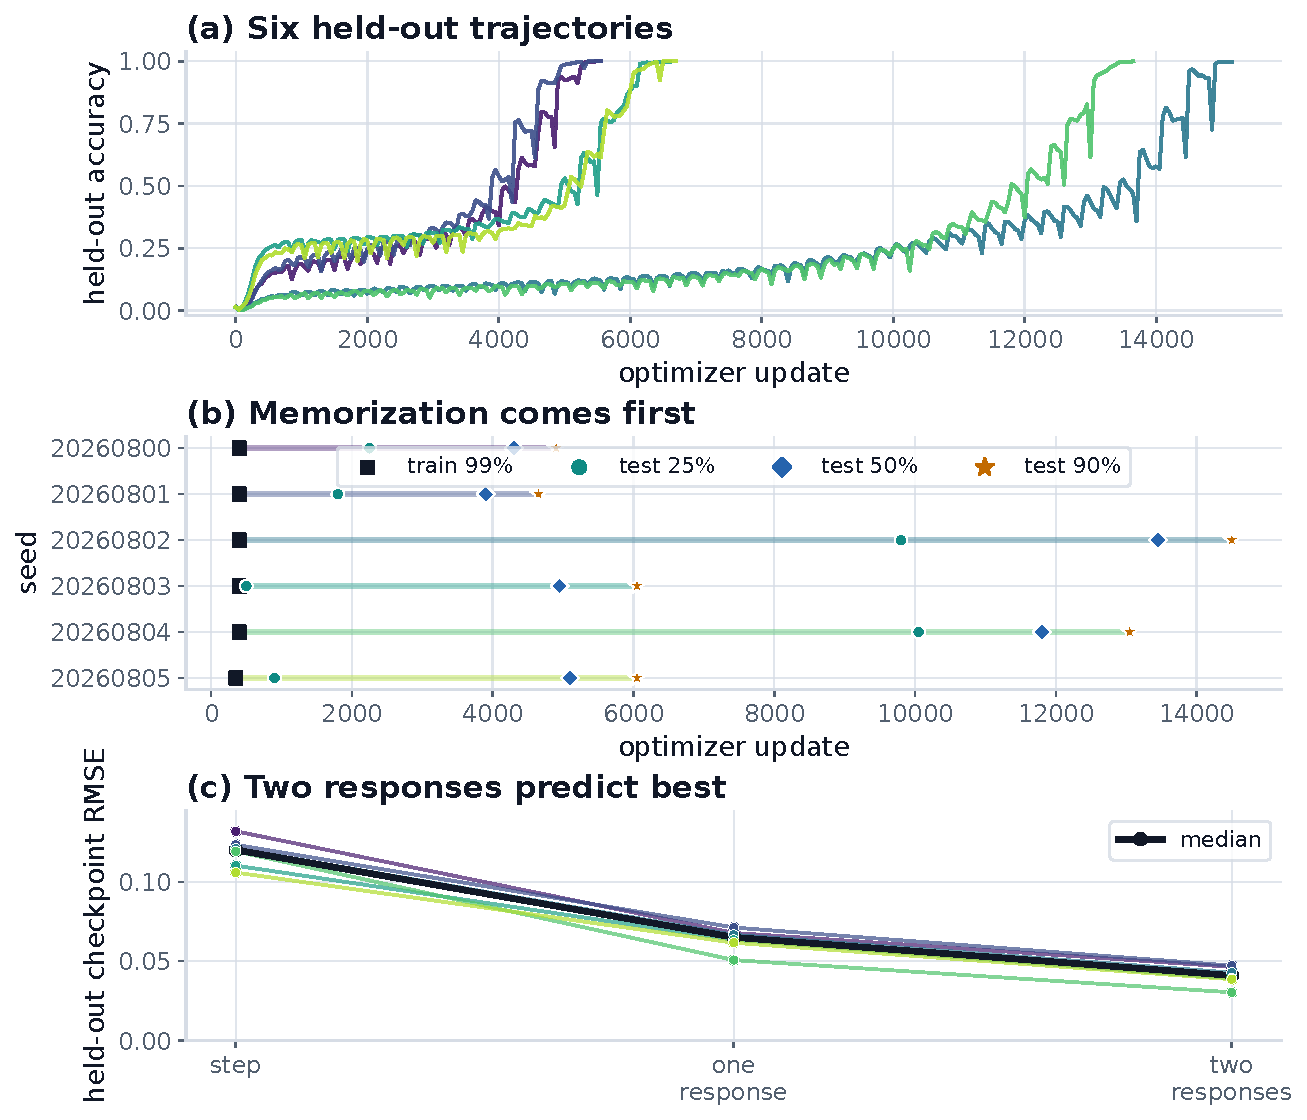
\includegraphics[width=0.94\linewidth]{experiment/runs/llm-takeoff-20260721T022627Z/results/trajectory_results_overview.pdf}
\caption{\textbf{The overall experiment.} (a) Held-out accuracy for six
confirmation seeds. (b) Training accuracy reaches 99 percent hundreds to
thousands of updates before held-out thresholds; the 50--90 percent segment
itself spans many checkpoints. (c) Checkpoint-level cross-validated error falls
for every seed from a step, to one smooth response, to two responses.}
\label{fig:overview}
\end{figure}

The first empirical fact is delay. Training accuracy reached 99 percent at
update 350 or 400 in every seed. Held-out accuracy did not reach 50 percent
until updates 3,900--13,450. The system had already fit its observed examples;
what followed was the delayed appearance of a rule on unseen pairs.

The second fact is width. From the first observed 50 percent accuracy to the
first observed 90 percent took 600--1,250 updates, with median 1,000. At
50-update spacing, the visibly steep final rise alone occupies 12--25 resolved
intervals. The full isotonic bounded-response kernel is broader still: its
10--90 percent mass width is 4,262--9,611 updates, with median 5,781 and a
median effective support of 23.5 checkpoints.

\begin{table}[H]
\centering
\small
\begin{tabular}{lccc}
\toprule
Quantity & Minimum & Median & Maximum\\
\midrule
Training 99\% step & 350 & 400 & 400\\
Held-out 50\% step & 3,900 & 5,025 & 13,450\\
Observed 50--90\% width & 600 & 1,000 & 1,250\\
Full-kernel 10--90\% width & 4,262 & 5,781 & 9,611\\
Effective kernel checkpoints & 19.4 & 23.5 & 29.9\\
\bottomrule
\end{tabular}
\caption{Resolved timing over six confirmation seeds. Widths are optimizer
updates; the observation spacing is 50 updates.}
\label{tab:timing}
\end{table}

Thus \emph{sudden} is true only comparatively: the last rise is short beside
the preceding delay. It is not instantaneous at the available resolution. The
takeoff impression comes from juxtaposing two timescales, not from a delta.

\section*{6. The jump is also composite}

Width alone does not explain the shape in Fig.~\ref{fig:overview}(a). Each
trajectory contains an early partial rise and a later completion. Under the
two-response fit, write
\[
F_i(t)=S\!\left(\frac{t-\tau_i}{s_i}\right),\qquad
\kappa_i(t)=\frac{dF_i}{dt}.
\tag{11}
\]
Then the fitted trajectory and its derivative obey the same mixture law:
\[
\widehat F(t)=\pi F_1(t)+(1-\pi)F_2(t),
\qquad
\widehat\kappa(t)=\pi\kappa_1(t)+(1-\pi)\kappa_2(t).
\tag{12}
\]
The final trajectory is therefore literally the cumulative sum of two
weighted finite-response kernels. No separate metaphor is needed: integrating
the right side of (12) gives the two-stage curve.
Figure~\ref{fig:composition} displays that identity directly: the cumulative
components add in panel (b), and their differentiated kernels add in panel (c).

\begin{figure}[!t]
\centering
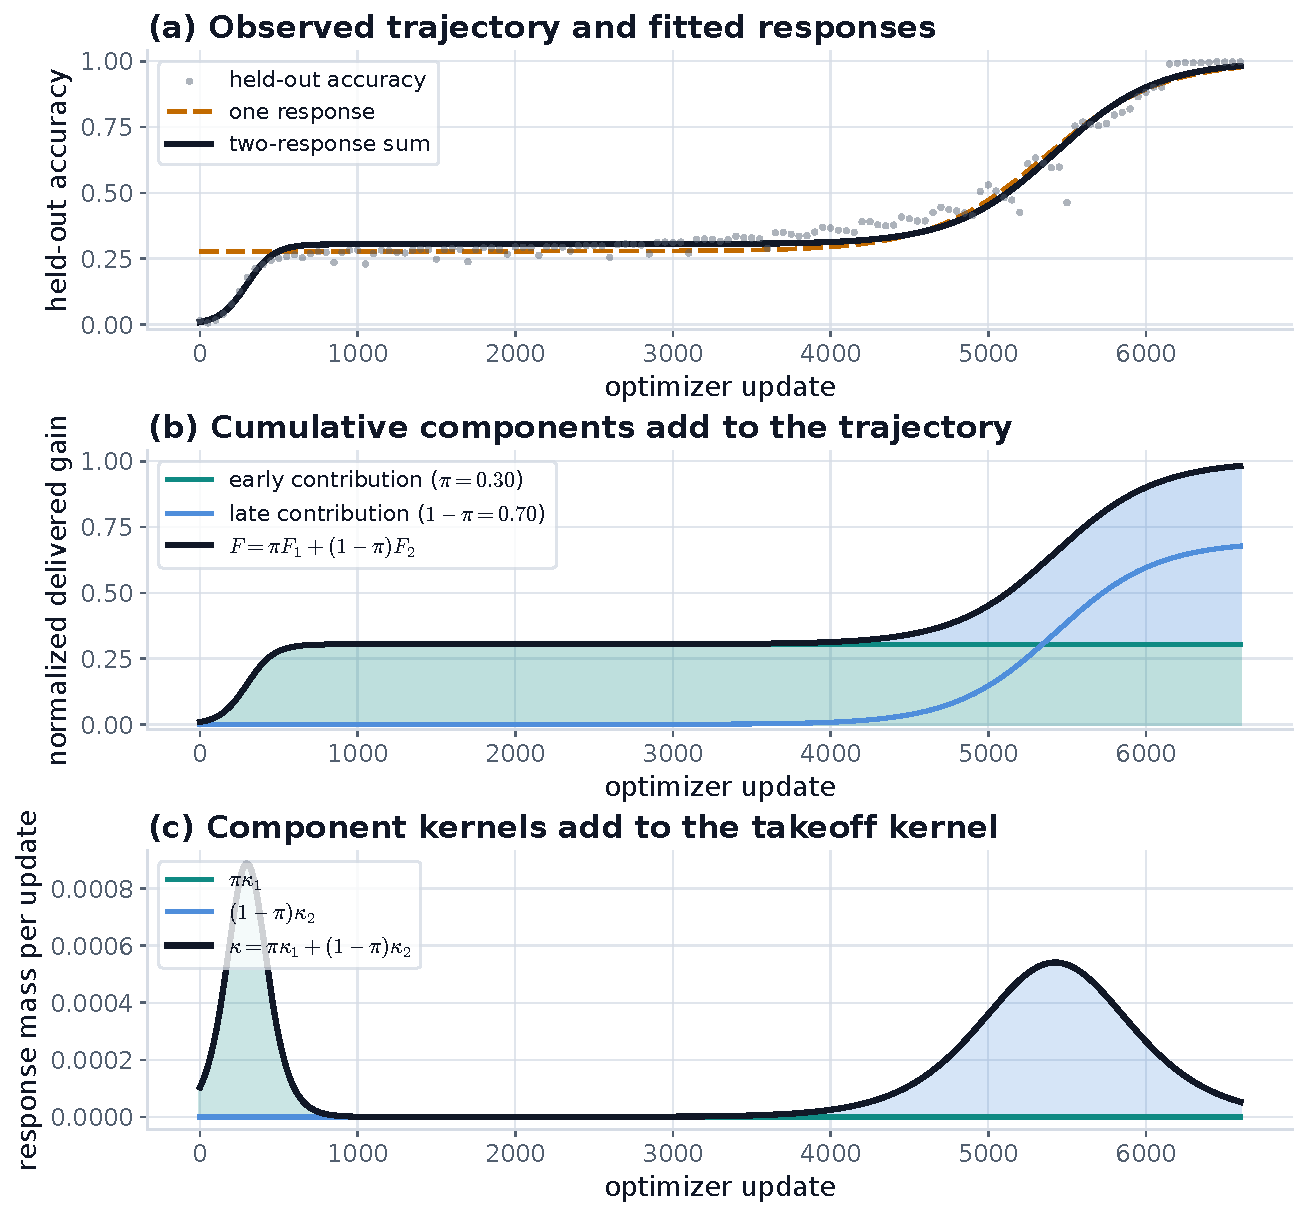
\includegraphics[width=0.94\linewidth]{experiment/runs/llm-takeoff-20260721T022627Z/results/kernel_composition_representative.pdf}
\caption{\textbf{Anatomy of the fitted response.} (a) For representative seed
20260803, one response absorbs the early plateau into a baseline; two responses
follow the data. (b) The early and late cumulative contributions add to the
normalized trajectory. (c) Their weighted kernels add pointwise to the final
takeoff kernel. This is the parallel mixture (6), not a demonstrated
sequential convolution (7).}
\label{fig:composition}
\end{figure}

For the representative seed, the early component is centered at update 298
and carries 30.5 percent of the response; the late component is centered at
5,424 and carries 69.5 percent. Across all seeds, early mass ranges from
26.5 to 40.4 percent, with median 30.2 percent. The component centers are
separated by 3,128--5,126 updates (median 3,824). The early component varies
from sharp to highly diffuse, while the late component is strikingly more
stable: its fitted 10--90 percent width lies between 1,193 and 1,441 updates
in every seed.

\begin{table}[H]
\centering
\small
\begin{tabular}{lccc}
\toprule
Trajectory model & Parameters & Held-out checkpoint RMSE & BIC wins\\
\midrule
Delta step & 3 & 0.106--0.132 & 0/6\\
One logistic response & 4 & 0.051--0.071 & 0/6\\
Two-response mixture & 7 & \textbf{0.030--0.047} & \textbf{6/6}\\
\bottomrule
\end{tabular}
\caption{Predictive comparison. RMSE is evaluated on alternating checkpoints
excluded from fitting; BIC treats checkpoints, not repeated evaluation items,
as longitudinal observations.}
\label{tab:models}
\end{table}

The mixture is favored by both checkpoint BIC and held-out checkpoint RMSE in
all six seeds. Yet a different question receives a negative answer. We fit one
and two decaying exponentials to the post-onset residual over both the full
tail and a local 5--95 percent window. The penalized fit selects one mode in
all 12 comparisons. The data support two separated \emph{arrivals} of
generalization, not two exponential tail modes. That negative result is useful:
it locates the extra structure in the response mixture rather than multiplying
hidden mechanisms without evidence.

\section*{7. What the experiment changes}

The strongest claim is narrow enough to be defensible and broad enough to
matter:

\begin{quote}
\emph{In this controlled language model, apparent takeoff is the terminal lobe
of a temporally extended, two-stage generalization response. It is neither an
instantaneous transition nor well summarized by one smooth onset.}
\end{quote}

The claim is novel within this framework because it joins two facts that are
usually reported separately. Grokking establishes a delay between memorization
and generalization. Finite-response analysis resolves what happens \emph{inside}
that delayed transition: about one-third of the eventual held-out gain arrives
through an earlier component, while a later, comparatively stable kernel
delivers the rest. A single \emph{grokking time} marks the most visible lobe and
misses the response already in motion.

This suggests a sharper reading of LLM scaling curves. A terminal exponent is
dynamically incomplete; a changepoint is temporally incomplete. Reporting a
kernel adds center, width, entropy, and internal composition. It also forces
the observation scale into the claim: a response may be delta-like at coarse
resolution and plainly finite at dense resolution.

The experiment does not establish a universal LLM kernel. It uses one small
architecture, one synthetic task, one pilot-selected hyperparameter condition,
and six seeds. Alternating checkpoint validation reduces but does not remove
temporal dependence. The logistic components are an economical descriptive
basis, not discovered neurons or circuits. Most importantly, a mixture fit does
not prove two physical channels. Distinguishing mixture from convolution, or
assigning components to memorization, representation formation, and rule
deployment, requires interventions and intermediate-state measurements.

The next decisive test is therefore comparative rather than merely larger:
predeclare the coordinate and estimators, then vary task family, data fraction,
regularization, depth, width, and model scale. If centered kernels collapse,
the common shape becomes a candidate universality class. If the approximately
30/70 split or the stable late width persists, it becomes a law worth
explaining. If not, the kernel still does its job: it shows exactly how the
route differs when the endpoint does not.

\section*{8. Conclusion}

An asymptote tells us where a learning curve is going. A finite-response kernel
tells us how it arrives. In the experiment here, the celebrated late jump is
real, but it is not singular and it is not alone. Generalization begins earlier,
travels through a broad first component, and completes through a sharper second
one. The interesting scientific object is not the instant of takeoff. It is the
resolved structure hidden by calling the whole journey a jump.

\vspace{0.35em}
{\footnotesize
\begin{thebibliography}{9}
\setlength{\itemsep}{0.05em}
\bibitem{kaplan2020}
J. Kaplan et al., "Scaling Laws for Neural Language Models," arXiv:2001.08361,
2020.
\bibitem{hoffmann2022}
J. Hoffmann et al., "Training Compute-Optimal Large Language Models,"
\emph{NeurIPS}, 2022.
\bibitem{power2022}
A. Power, Y. Burda, H. Edwards, I. Babuschkin, and V. Misra, "Grokking:
Generalization Beyond Overfitting on Small Algorithmic Datasets," \emph{ICLR},
2022.
\end{thebibliography}
}

\end{document}
